\documentclass[a4paper, 12pt, titlepage]{report}
\usepackage{minted}
\usepackage[dvipsnames]{xcolor}
\colorlet{LightApricot}{Orchid!20}
\usepackage{graphicx}
\usepackage{fullpage}
\usepackage{float}
\usepackage{hyperref}
%\usepackage{longtable}
%\usepackage{amsmath}
%\usepackage[normalem]{ulem}
\usepackage{booktabs}
\usepackage{dirtree}
\usepackage{hologo}
%\usepackage{array}
%\usepackage{tikz}
%\usepackage{parskip}
%\newcommand{\tabitem}{~~\llap{\textbullet}~~}
\setlength{\tabcolsep}{18pt}
\renewcommand{\arraystretch}{1.5}
\renewcommand{\chaptername}{Section}
\hypersetup{
    colorlinks=true,
    linkcolor=blue,
    filecolor=magenta,      
    urlcolor=RoyalBlue,
}
\begin{document}
\linespread{1.25}
\author{Affaan Muhammad - 33016763\\Joshua Esterhuizen - 30285976}
\title{ITRI615 - Computer Security\\Project Documentation}
\date{}
\maketitle
\tableofcontents{}

\chapter{Installation and setup}
\section{Project files}
The project files can be found on the following GitHub link:\\
\url{https://github.com/AM-ops/SecurityProject}
\\\\This was our main code repository. We both have been updating the code as we went along and added details and bug fixes to the project.\\\\
To copy the code to your own machine, follow the following steps:
\begin{enumerate}
\item Make sure Git is installed. If not it can be downloaded from here:\\
\url{https://git-scm.com/}
\item Create an empty directory where the code can be copied to
\item Run the following command:
\begin{minted}
[
frame=lines,
framesep=2mm,
baselinestretch=1.2,
bgcolor=LightApricot,
fontsize=\footnotesize,
]
{Shell}
git clone https://github.com/AM-ops/SecurityProject.git
\end{minted}
\end{enumerate}
\section{Virtual Environment}
There are multiple advantages of using virtual environments when creating software. The primary reason being we create a layer of separation and abstraction between our host machine's files and our software project.\\\\
We made use of a Python virtual environment which was handled by Anaconda. This can be downloaded from the following link:\\
\url{https://www.anaconda.com/products/individual}
\subsection{Creating a virtual environment}
Once Anaconda was installed the following commands were run in the terminal to create a virtual environment called \texttt{myDjangoEnv}.
\begin{minted}
[
frame=lines,
framesep=2mm,
baselinestretch=1.2,
bgcolor=LightApricot,
fontsize=\footnotesize,
]
{Shell}
conda create --name myDjangoEnv
\end{minted}
Depending on the version of Anaconda installed you might have to use a leading underscore on Windows machines. The same will apply for commands further down. Below is a demonstration.
\begin{minted}
[
frame=lines,
framesep=2mm,
baselinestretch=1.2,
bgcolor=LightApricot,
fontsize=\footnotesize,
]
{Shell}
_conda create --name myDjangoEnv
\end{minted}
\subsection{Listing virtual environments}
To list all virtual environments on your host machine run the following command.
\begin{minted}
[
frame=lines,
framesep=2mm,
baselinestretch=1.2,
bgcolor=LightApricot,
fontsize=\footnotesize,
]
{Shell}
conda info --envs
\end{minted}
or
\begin{minted}
[
frame=lines,
framesep=2mm,
baselinestretch=1.2,
bgcolor=LightApricot,
fontsize=\footnotesize,
]
{Shell}
conda env list
\end{minted}
\subsection{Deleting a virtual environment}
To delete a virtual environment run the following commands.
\begin{minted}
[
frame=lines,
framesep=2mm,
baselinestretch=1.2,
bgcolor=LightApricot,
fontsize=\footnotesize,
]
{Shell}
conda remove --name <name_of_virtual_environment> --all
\end{minted}
or
\begin{minted}
[
frame=lines,
framesep=2mm,
baselinestretch=1.2,
bgcolor=LightApricot,
fontsize=\footnotesize,
]
{Shell}
conda env remove --name <name_of_virtual_environment>
\end{minted}
\subsection{Activating and deactivating virtual environments}
To activate an environment run the following commands for Windows.
\begin{minted}
[
frame=lines,
framesep=2mm,
baselinestretch=1.2,
bgcolor=LightApricot,
fontsize=\footnotesize,
]
{Shell}
conda activate <name_of_virtual_environment>
\end{minted}
For Linux and MacOS the command is as follows.
\begin{minted}
[
frame=lines,
framesep=2mm,
baselinestretch=1.2,
bgcolor=LightApricot,
fontsize=\footnotesize,
]
{Shell}
source activate <name_of_virtual_environment>
\end{minted}
Once the environment is activated your terminal should change. By default, the active environment, is shown in parentheses () or brackets [] at the beginning of your command prompt as shown below.
\begin{minted}
[
frame=lines,
framesep=2mm,
baselinestretch=1.2,
bgcolor=LightApricot,
fontsize=\footnotesize,
]
{Shell}
(<name_of_virtual_environment>) >_
\end{minted}
Depending on your version of Anaconda to deactivate your environment the commands for Windows is.
\begin{minted}
[
frame=lines,
framesep=2mm,
baselinestretch=1.2,
bgcolor=LightApricot,
fontsize=\footnotesize,
]
{Shell}
deactivate
\end{minted}
or
\begin{minted}
[
frame=lines,
framesep=2mm,
baselinestretch=1.2,
bgcolor=LightApricot,
fontsize=\footnotesize,
]
{Shell}
conda deactivate
\end{minted}
For Linux and MacOS the command will be
\begin{minted}
[
frame=lines,
framesep=2mm,
baselinestretch=1.2,
bgcolor=LightApricot,
fontsize=\footnotesize,
]
{Shell}
source deactivate
\end{minted}
\subsection{Listing Packages installed}
To list all the packages you have installed in an environment there are two methods of listing them.
First, if the environment is not activated run the following.
\begin{minted}
[
frame=lines,
framesep=2mm,
baselinestretch=1.2,
bgcolor=LightApricot,
fontsize=\footnotesize,
]
{Shell}
conda list -n <name_of_virtual_environment>
\end{minted}
Secondly, if the environment is activated, then simply run the following.
\begin{minted}
[
frame=lines,
framesep=2mm,
baselinestretch=1.2,
bgcolor=LightApricot,
fontsize=\footnotesize,
]
{Shell}
conda list
\end{minted}
\subsection{Using pip}
Due to the fact that Python is being used for the project it is always necessary to make sure \texttt{pip} is installed and functioning. If it is not then run the following commands.
\begin{minted}
[
frame=lines,
framesep=2mm,
baselinestretch=1.2,
bgcolor=LightApricot,
fontsize=\footnotesize,
]
{Shell}
conda install -n <name_of_virtual_environment> pip
\end{minted}
\section{Frameworks and other packages}
\subsection{Django}\label{dj}
The primary framework used for development in this project was \texttt{Django}. This is a python based Web framework. The documentation for it can be found here:\\
\url{https://docs.djangoproject.com/en/3.2/}
\subsection{Bootstrap}\label{bs}
Bootstrap is Cascading Style Sheets (CSS) Framework which allows for simple, elegant, and responsive Graphical User Interfaces to be developed for the Web. The documentation for it can be found here:\\
\url{https://getbootstrap.com/docs/5.0/getting-started/introduction/}\\\\
For a more seamless integration of Bootstrap with the \texttt{Django} Framework an additional package called \texttt{django-crispy-forms} was also installed. Its documentation ca be found here:\\
\url{https://django-crispy-forms.readthedocs.io/en/latest/}
\subsection{Miscellaneous}
For typesetting of this documentation, \hologo{LaTeX} was utilised. Additionally, a \hologo{LaTeX} package called \texttt{minted} was used to typeset code in this documentation. Its homepage is located at: \url{https://www.ctan.org/pkg/minted}\\
To typeset directory structures in a tree-like manner the \hologo{LaTeX} package \texttt{dirtree} was used. Its homepage can be found at: \url{https://ctan.org/pkg/dirtree}\\\\
Lastly, to typeset code within the HTML pages of our project the JavaScript library called \texttt{Rainbow} was implemented. The GitHub link for that is located at:\\
\url{https://github.com/ccampbell/rainbow}
\chapter{Programming of artefact}
\section{Development Tools}
\subsection{Operating Systems}
The primary systems on which development was done was Linux and Windows 10. The same systems where utilised for testing and bug fixing purposes.
\subsection{IDEs}
For the purposing of coding the following two Integrated Development Environments were used:
\begin{enumerate}
\item Atom. It can be downloaded from: \url{https://atom.io/}
\item Visual Studio Code, also known as VSCode. It can be downloaded from here: \url{https://code.visualstudio.com/}
\end{enumerate}
\subsection{Database Management Tools}
For the purposes of database management, TablePlus was the main software we utilised. It was used to see if our \texttt{Django} models and cryptographic schemes were correctly implemented. TablePlus can be downloaded from: \url{https://tableplus.com/}
\subsection{Hosting}
Due to a number of constraints we landed up running our project locally. The server was \texttt{localhost} and the port number was \texttt{8000}. Therefore the link where we ran our project was:
\url{http://127.0.0.1:8000}
\section{Prerequisites}
\subsection{Project and Package Initialisation}
\textsl{From here on we will refer to the working directory as the directory where the} \texttt{manage.py} \textsl{file is located. This file is created when the project is setup}\\\\
Before our \texttt{Django} project can be created we have to install all the packages mentioned above in Section \ref{dj} and \ref{bs}. A text file called \texttt{requirements.txt} was created which lists the 3 packages we need to install as shown below:
\begin{minted}
[
frame=lines,
framesep=2mm,
baselinestretch=1.2,
bgcolor=LightApricot,
fontsize=\footnotesize,
]
{Text}
django
django-crispy-forms
bootstrap4
\end{minted}
Thereafter the following command was run in the working directory.
\begin{minted}
[
frame=lines,
framesep=2mm,
baselinestretch=1.2,
bgcolor=LightApricot,
fontsize=\footnotesize,
]
{Shell}
pip install -r requirements.txt
\end{minted}
To start a \texttt{Django} project called \texttt{SecProj} the following command was run:
\begin{minted}
[
frame=lines,
framesep=2mm,
baselinestretch=1.2,
bgcolor=LightApricot,
fontsize=\footnotesize,
]
{Shell}
django-admin startproject SecProj
\end{minted}
Your directory should look like the following:
\dirtree{%
.1 /.
.2 manage.py.
.2 SecProj.
.3 \_\_init\_\_.py.
.3 settings.py.
.3 urls.py.
.3 asgi.py.
.3 wsgi.py.
}
\phantom{a}\\
\noindent To verify that your \texttt{Django} project is working run the following command in your working directory:
\begin{minted}
[
frame=lines,
framesep=2mm,
baselinestretch=1.2,
bgcolor=LightApricot,
fontsize=\footnotesize,
]
{Shell}
python manage.py runserver
\end{minted}
You should see the following if you open the link: \url{http://127.0.0.1:8000}
\begin{figure}[H]
\centering
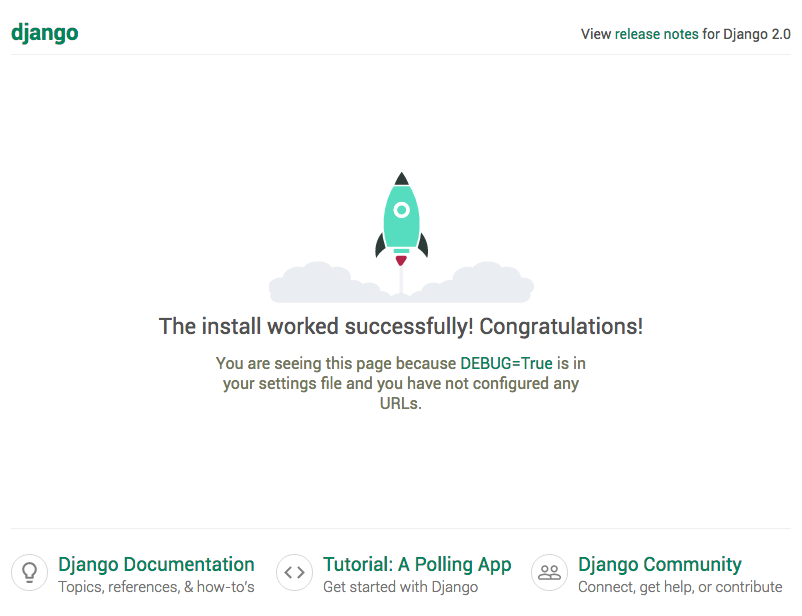
\includegraphics[scale=0.3]{./pics/home}
\caption{Default Homepage of a new Django Project}
\end{figure}
\noindent Now that your \texttt{Django} project is up and running it is time to create a \texttt{Django} 'App' within this project. This App is where we implemented our cryptographic schemes and the bulk of our project. We called our App \texttt{SecApp} and the command to run in your working directory is as follows:
\begin{minted}
[
frame=lines,
framesep=2mm,
baselinestretch=1.2,
bgcolor=LightApricot,
fontsize=\footnotesize,
]
{Shell}
python manage.py startapp SecApp
\end{minted}
Your directory should now look like the following:
\dirtree{%
.1 /.
.2 manage.py.
.2 SecProj.
.3 \_\_init\_\_.py.
.3 settings.py.
.3 urls.py.
.3 asgi.py.
.3 wsgi.py.
.2 SecApp.
.3 \_\_init\_\_.py.
.3 admin.py.
.3 apps.py.
.3 migrations.
.4 \_\_init\_\_.py.
.3 models.py.
.3 tests.py.
.3 views.py.
}
\subsection{Settings and Admin}
\chapter{User manual}
\chapter{Reflection}
\chapter{Sources}
\url{https://conda.io/projects/conda/en/latest/user-guide/tasks/manage-environments.html}\\
\url{https://www.udemy.com/course/python-and-django-full-stack-web-developer-bootcamp/}\\
\url{https://docs.djangoproject.com/en/3.2/}
\end{document}